\documentclass[a4paper,11.9pt]{article}
\usepackage[a4paper, mag=1000, left=2cm, right=2cm, top=2cm, bottom=2cm, headsep=0.7cm, footskip=1cm]{geometry}
\usepackage[utf8]{inputenc}
\usepackage[english,russian]{babel}
\usepackage{indentfirst}
\usepackage[dvipsnames]{xcolor}
\usepackage[colorlinks]{hyperref}
\usepackage[argument]{graphicx}
\DeclareGraphicsExtensions{.pdf,.png,.jpg}
\usepackage{listings} 
\usepackage{caption}
\usepackage{amsmath}
\DeclareCaptionFont{white}{\color{white}} 
\DeclareCaptionFormat{listing}{\colorbox{gray}{\parbox{\textwidth}{#1#2#3}}}
\captionsetup[lstlisting]{format=listing,labelfont=white,textfont=white}
\lstset{% Собственно настройки вида листинга
inputencoding=utf8, extendedchars=\true, keepspaces = true, % поддержка кириллицы и пробелов в комментариях
language=Pascal,            % выбор языка для подсветки (здесь это Pascal)
basicstyle=\small\sffamily, % размер и начертание шрифта для подсветки кода
numbers=left,               % где поставить нумерацию строк (слева\справа)
numberstyle=\tiny,          % размер шрифта для номеров строк
stepnumber=1,               % размер шага между двумя номерами строк
numbersep=5pt,              % как далеко отстоят номера строк от подсвечиваемого кода
backgroundcolor=\color{white}, % цвет фона подсветки - используем \usepackage{color}
showspaces=false,           % показывать или нет пробелы специальными отступами
showstringspaces=false,     % показывать или нет пробелы в строках
showtabs=false,             % показывать или нет табуляцию в строках
frame=single,               % рисовать рамку вокруг кода
tabsize=2,                  % размер табуляции по умолчанию равен 2 пробелам
captionpos=t,               % позиция заголовка вверху [t] или внизу [b] 
breaklines=true,            % автоматически переносить строки (да\нет)
breakatwhitespace=false,    % переносить строки только если есть пробел
escapeinside={\%*}{*)}      % если нужно добавить комментарии в коде
}
\usepackage{setspace}
 \setstretch{1.2}
\begin{document}
% Переоформление некоторых стандартных названий
\renewcommand{\chaptername}{Лабораторная работа}
\def\contentsname{Содержание}

% Оформление титульного листа
\begin{titlepage}\large
\begin{center}
\textsc{Московский государственный университет\\
имени М.И.Ломоносова\\[5mm]
Механико-математический факультет\\[5cm]
}


\Large\textbf{Отчет по задаче № 1\\[4mm]
Численное решение краевой задачи методом конечных разностей\\[7mm]
\\[19mm]
}
\end{center}

\vfill
\begin{flushright}
\begin{minipage}{0.25\textwidth}
\begin{flushleft}
Выполнил студент:\\[2mm] 
Хисамеев О.В.\\
группа: 404\\[5mm]
\end{flushleft}
\end{minipage}
	
\end{flushright}%
\vfill
\begin{center}
 Москва, 2022 г.
\end{center}
\end{titlepage}
\newpage

\section*{\centering Постановка задачи} \Large
Построить разностную схему со вторым порядком аппроксимации и найти ее решение при различных значениях $h$ и $\alpha$:
\begin{gather}
-u^{\prime\prime} + e^u = \alpha \cdot sin(x^2),\label{1}\\
u(0) = u(1) = 0, \; \alpha = 0.1, 1, 10.\notag
\end{gather}
\section*{\centering Алгоритм выполнения задачи} \Large
Для начала опишем метод конечных разностей. Разобьем отрезок $[0, 1]$ на $n$ равных частей. Обозначим через $h = \frac{1}{n}$ - шаг полученного разбиения, $x_i$ - точки разбиения: 
\begin{equation}
узловые x_i = i\cdot h, \; \; где\;  i = 0, \ldots, n \label{2}
\end{equation}
Будем искать приближенное решение задачи $(\ref{1})$ в узловых точках разбиения отрезка $x_i, \; i = 1, \ldots, n - 1$ ($x_0 = x_n = 0$). \\
Выражения 
\begin{gather}
    u^\prime \approx \frac{u(x + h) - u(x - h)}{h},\label{3}\\
    u^{\prime\prime} \approx \frac{u(x + h) - 2u(x) + u(x - h)}{h^2}\label{4}
\end{gather}
называются \textit{конечно-разностной аппроксимацией} соответствующих производных. Чтобы выяснить насколько хорошо правые части (\ref{3}) и (\ref{4}) аппроксимируют производные, воспользуемся разложением Тейлора
\begin{gather}
    u(x + h) = u(x) + u^\prime(x)h + \frac{1}{2!}u^{\prime \prime}(x)h^2 + \frac{1}{3!}u^{(3)}(x)h^3 + O(h^4)\label{5}\\
    u(x - h) = u(x) - u^\prime(x)h + \frac{1}{2!}u^{\prime \prime}(x)h^2 - \frac{1}{3!}u^{(3)}(x)h^3 + O(h^4).\label{6} 
\end{gather}
Из (\ref{5}) и (\ref{6}) немедленно получаем:
\begin{gather}
u^\prime(x) - \left[\frac{u(x + h) - u(x)}{h} \right] = -\frac{1}{2}u^{\prime \prime}(x) - \frac{1}{3!}u^{(3)}(x)h^2 + O(h^3)\label{7}\\
u^\prime(x) - \left[\frac{u(x) - u(x - h)}{h} \right] = \frac{1}{2}u^{\prime \prime}(x) - \frac{1}{3!}u^{(3)}(x)h^2 + O(h^3).\label{8}
\end{gather}
Сложив и разделив на 2 равенства (\ref{7}) и (\ref{8}), получаем
\begin{equation}
    u^\prime(x) - \left[\frac{u(x + h) - u(x - h)}{2h} \right] = - \frac{1}{2\cdot 3!}u^{(3)}(x)h^2 + O(h^3),
\end{equation}
откуда видно, что аппроксимация имеет второй порядок. Аналогично определяется погрешность аппроксимации (\ref{4}), также пропорциональная $h^2$.\\
Далее будем использовать следующее обозначение 
\begin{center}
$u_i = u(x_i)$, для \;$i = 0, \ldots, n.$
\end{center}
Здесь $x_i  $ являются точками разбиения отрезка $[0, 1]$ (см. (\ref{2})).\\
Запишем граничные условия в этих обозначениях:\\
\begin{equation*}
\begin{cases}
    u_0 = 0\\
    u_n = 0\\
    \end{cases}    
\end{equation*}
Если теперь подставить полученные приближения в уравнение (\ref{1}), то получим 
\begin{equation}
    \begin{cases}
        u_{i+1} - 2u_i + u_{i-1} = h^2 \cdot (e^{u_i} - \alpha sin(x_i^2))\\
        u_0 = u_n = 0
    \end{cases}
\end{equation}
 Уравнения (10) представляют собой систему $n - 2$ нелинейных уравнений относительно $n - 2$ неизвестной $u_2, \ldots, u_{n - 1}.$ Перепишем ее в следующей матричной форме, учитывая граничные условия:\\
 
\begin{equation}
    Au + H(u) = 0, \; \text{где}\\
\end{equation}

\begin{equation}
    A = 
    \begin{pmatrix}
        2& -1& 0&  \ldots& 0& 0&\\
        -1& 2& -1&  \ldots& 0& 0&\\
        0& -1& 2& \ldots& 0& 0&\\
        \ldots& \ldots& \ldots& \ldots& \ldots& \ldots&\\
        0& 0& 0& \ldots& 2& -1&\\
        0& 0& 0& \ldots& -1& 2&\\
    \end{pmatrix}
    \quad
    u = 
    \begin{pmatrix}
        u_1\\
        u_2\\
        \ldots&\\
        u_{n-1}\\
    \end{pmatrix}
\end{equation}

\begin{equation}
    H(u) = h^2 \cdot
    \begin{pmatrix}
        e^{u_1} - \alpha sin(x_1^2)&\\
        e^{u_2} - \alpha sin(x_2^2)&\\
        \ldots&\\
        e^{u_{n-1}} - \alpha sin(x_{n-1}^2)&\\
    \end{pmatrix}
\end{equation}

Таким образом, задача сводится к решению этой системы нелинейных уравнений, решение которой и будет значением решения поставленной задачи в точках $x_i$ для $i = 1,\ldots,n-1$.\\
Решать систему (11) будем методом Ньютона. k-я итерация метода Ньютона решения системы нелинейных уравнений состоит в следующем:
\begin{enumerate}
    \item Решить систему линейных уравнений $[A + H'(u^k)]y^k = -[Au^k + H(u^k)]$;
    \item Положить $u^{k+1} = u^k + y^k$, где $H'(u)$ - матрица якоби для $H$:
\end{enumerate}

\begin{equation}
    H' = h^2 \cdot
    \begin{pmatrix}
        e^{u_1}& 0&  \ldots& 0& 0&\\
        0& e^{u_2}&  \ldots& 0& 0&\\
        \ldots& \ldots& \ldots& \ldots& \ldots&\\
        0& 0&  \ldots& e^{u_{n-2}}& 0&\\
        0& 0& \ldots& 0& e^{u_{n-1}}&\\
    \end{pmatrix}
\end{equation}

Для первой итерации инициализируем $u$ нулями.
Алгоритм заканчивает свою работу, когда норма $y$ становится меньше заранее установленной величины $\varepsilon$.

Данный алгоритм решения линейной системы уравнений реализован мною на языке программирования python с использованием модулей numpy, pandas, matplotlib и seaborn.
\newpage
\section*{\centering Результаты} \Large 
Ниже приведены графики численных приближений решений задачи (\ref{1}).

\begin{figure}[h]
    \center{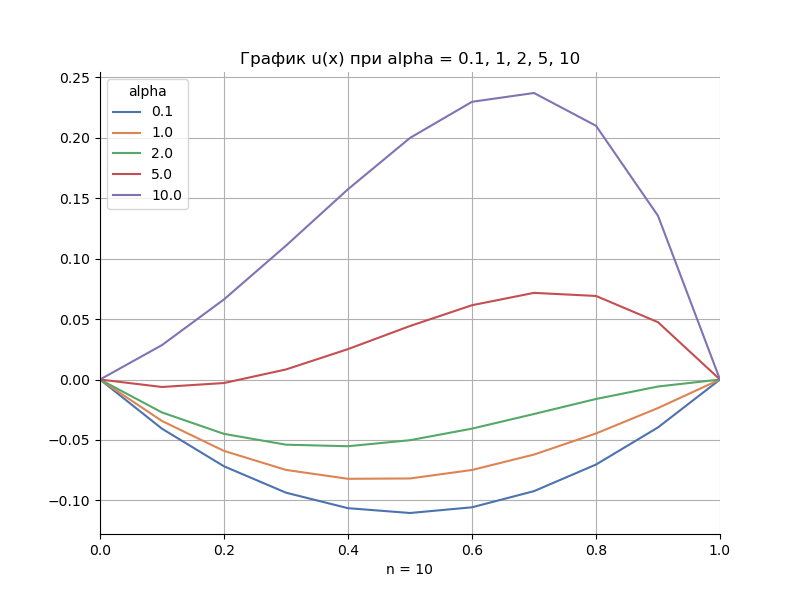
\includegraphics[scale=0.62]{n(10)_alpha(0.1,1,2,5,10).png}}
    \label{fig:image}
\end{figure}


\begin{figure}[h]
    \center{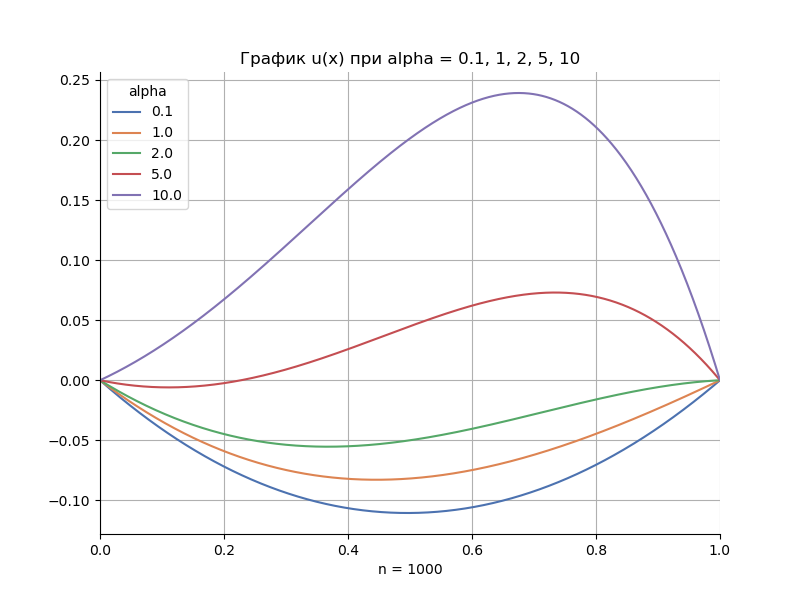
\includegraphics[scale=0.62]{n(1000)_alpha(0.1,1,2,5,10).png}}
    \label{fig:image}
\end{figure}

\newpage

\begin{figure}[h]
    \center{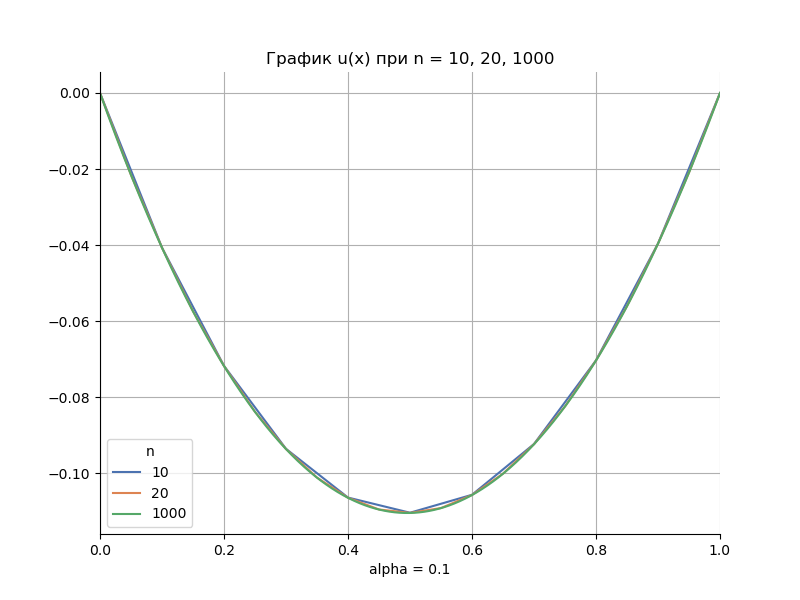
\includegraphics[scale=0.85]{alpha(0.1)_n(10,20,1000).png}}
    \label{fig:image}
\end{figure}

\newpage

\begin{figure}[h]
    \center{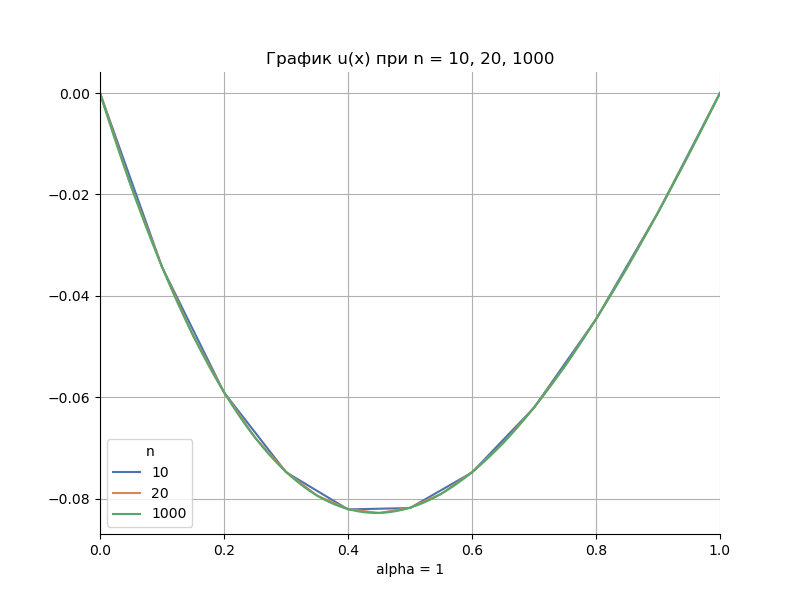
\includegraphics[scale=0.85]{alpha(1)_n(10,20,1000).png}}
    \label{fig:image}
\end{figure}

\newpage

\begin{figure}[h]
    \center{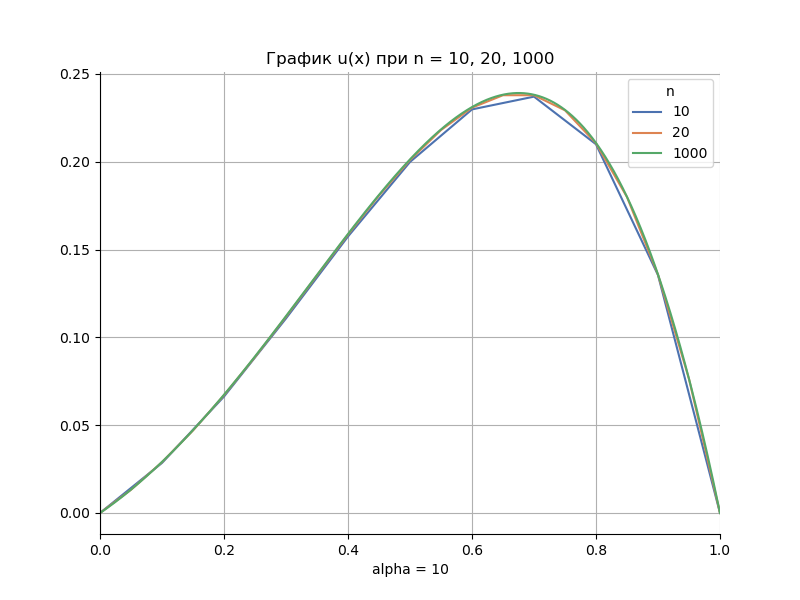
\includegraphics[scale=0.85]{alpha(10)_n(10,20,1000).png}}
    \label{fig:image}
\end{figure}

\newpage

\section*{ Список литературы:} 
 \begin{enumerate}
     \item \textit{Ортега Дж., Пул У.} Введение в численные методы решения дифференциальных уравнений.
     \item \textit{Бахвалов Н. С., Корнев А.А., Чижонков Е.В. } Численные методы решения задач и упражения.
     \item \textit{Бахвалов Н. С., Жидков Н.П., Кобельков Г.М. } Численные методы.
 \end{enumerate}
\end{document} % конец документа
